%%% Documentclass-Options:
\documentclass[11pt, iace, german]{bmim.paper} % Nichts ändern 

% Hier Versuchsname und Ihre Namen eingeben 
\articletitle{Hilfestellung: \\Aufbau eines Laborbericht} % To break lines in long titles use \\
\subarticletitle{Institut für Automatisierungs- und Regelungstechnik}
\authorlist{Thomas Auer}

\usepackage{amsmath}
\usepackage{siunitx}

%%%%%%%%%%%%%%%%%%%%%%%%%%%%%%%%%%%%%%%%%%%%%%%%%%%%%%%%
%%%
% * <hochers@web.de> 2018-07-27T06:04:24.310Z:
% ^.
%%%  Main document.
%%%
%%%  To span floating objects (wide images, tables, etc.)
%%%  over twocolumn layout, use figure*
%%%  or table* environments.
%%%
%%%  Examples:
%%%  \begin{figure*}	 \begin{table*}
%%%   ...				  ...
%%%  \end{figure*}		 \end{table*}
%%%
%%%%%%%%%%%%%%%%%%%%%%%%%%%%%%%%%%%%%%%%%%%%%%%%%%%%%%%%

\begin{document}
\maketitle

%-----Löschen Sie diesen Abschnitt  ---------------------
% Lesen Sie unbedingt die Grundlagen des wissenschaftlichen Arbeitens 
% bevor Sie einen Laborbericht schreiben!
\section*{Einleitung}
In der Einleitung wird die im Labor zu untersuchende Forschungsfrage kurz beschrieben. Für Ergebnisse (auch für Korrekte), welche nicht ausreichend beschrieben sind, werde keine Punkte vergeben. Um bei der Erstellung des Laborberichts zu helfen, ist diese Vorlage wie ein Laborbericht selbst aufgebaut (so gut es möglich war - es ist nicht an allen Stellen möglich, sollte aber dennoch klar sein). Mit diesem Dokument soll die Frage beantwortet werden, ob Studierende mit einer Anleitung umgehen können, die schon so aufgebaut ist, wie der Laborbericht selbst. Des weiteren ist dann klar, warum Berichte teilweise sehr schlecht bewertet werden, obwohl "da ja alles drin war". An sich soll der Laborbericht ein eigenständiges Dokument sein. Es muss möglich sein, alle Bearbeiteten Schritte nachvollziehen zu können. Es muss möglich sein den Gedankengängen der ErstellerInnen zu folgen. Vor allem muss es möglich sein den Laborbericht zu verstehen, \textbf{ohne} die Angabe des Labors zu kennen, oder beim Labor dabei gewesen zu sein. Am Ende der Einleitung befindet sich ein kurzer Überblick über die einzelnen Kapitel des Laborberichtes. In Abschnitt~\ref{sec:wissensch_schreiben} befindet sich eine kurze Beschreibung, wie die Struktur des Berichtes an sich sein sollte. Anschließend folgt eine Kurze Übersicht in Abschnitt~\ref{sec:mathematik}, welcher Bezug auf Mathematik gibt und die häufigsten Fehler aufzeigt. Ein Negativbeispiel, wie Beschreibungen nicht ausschauen sollen, befindet sich in Abschnitt~\ref{sec:negativbeispiel}. In Abschnitt~\ref{sec:bezug_zur_Angabe} befindet sich eine kurze plakative Beschreibung, wie ein Punkt im Laborbericht bearbeitet werden sollte.



\section{Aufbau/ Wissenschaftliches Schreiben}\label{sec:wissensch_schreiben}
Der erste Teil des Laborberichtes, die Einleitung, wurde bereits behandelt. Die folgenden Kapitel betreffen die restlichen Punkte selbst. Vorweg muss auf die Sprache im Laborbericht geachtet werden. Der Laborbericht dient der Dokumentation der durchgeführten Arbeiten und ist keine Ergebniserzählung. Die folgenden Punkte müssen beachtet werden \citep{Heesen.2014}:
\begin{itemize}
	\item Nicht in der \textit{Ich/Wir} Form schreiben
	\item Nicht erzählen: Anstelle von \textit{und als nächstes haben wir xyz gemessen} das folgende verwenden: \textit{im nächsten Schritt wurde xyz gemessen};
\end{itemize}
Für unvollständige Beschreibungen oder wenn die Laborangabe schlichtweg als Kopie eingefügt wird, werde gleich viele Punkte vergeben, wie für fehlende Abbildungen. Die erhaltene Punkteanzahl $P_{\text{erh}}$ dafür kann mit der Formel
\begin{equation}\label{eq:Punktezahl_fehlende_beschr}
	P_{\text{erh}} = 0 \cdot  n \qquad n \in \mathbb{N}
\end{equation}
berechnet werden. Geben sie alle Verwendeten Quellen an \citep{Umit_plag, Rettig.2017} und vermeiden Sie dadurch Plagiate. Abbildungen werden in der Laborangabe oft nicht explizit gefordert, sind aber oft Notwendig, um Sachverhalte erklären zu können. Werden einfach zu überprüfende Behauptungen aufgestellt wie: "Die Abweichungen zwischen Messung und Simulation kommen von einer Parameterabweichung der Federkonstante in der Simulation", sollte dies auch entsprechend gezeigt werden. Die Struktur des Laborberichts soll sich an der Angabe orientieren. Die Nummerierung muss nicht 1:1 gleich sein, soll aber die gleiche Struktur aufweisen. 



\section{Mathematische Beispiele}\label{sec:mathematik}
Die Punkteanzahl für fehlende Beschreibungen kann bereits mit \eqref{eq:Punktezahl_fehlende_beschr} berechnet werden. Formeln sollen wie die folgenden Beispiele im Text eingebaut werden. Was \textbf{nicht} extra beschrieben werden muss sind einfache Rechnungen, wie das Schrittweise auflösen einer Formel, wenn die notwendigen Schritte klar sind, oder das Invertieren einer Matrix. Ein häufiger Fehler ist die falsche Angabe höherer Ableitungen. Ist $x$ die Position, $\dot{x}$ die Geschwindigkeit und $\ddot{x}$ die Beschleunigung, dann werden alle noch höheren Ableitungen mit
\begin{equation}
	x^{\left(3\right)}, \ x^{\left(4\right)}, \ \dots
\end{equation}
angegeben. Die Zahl in der hochgestellten Klammer $x^{\left( \text{Zahl} \right)}$ bezeichnet hier den Grad der Ableitung. Eine Sonderstellung hat hier der Strom $i \! \left(t\right) $. Hier ist es übersichtlicher und besser, die Schreibweise
\begin{equation}
	\frac{d}{d t}i\! \left(t\right), \qquad \text{bzw.} \quad \frac{d^n}{d t^n}i\! \left(t\right)
\end{equation}
anstelle von $\dot{i}\! \left(t\right)$ zu verwenden. Verwenden Sie für Vektoren und Matrizen entsprechende Kennzeichnungen. Der Zustandsvektor $\bm{z} = \left[x, \ \dot{x}\right]^T$ wird zuerst eingeführt und damit kann ein Modell der Form
\begin{equation}\label{eq:bsp_modellgleichung}
	\dot{\bm{z}} = \bm{A} \, \bm{z} + \bm{b} \, u
\end{equation}
angegeben werden. Wobei $\bm{A}$ eine Matrix und $\bm{b}$ ein Vektor ist. Wenn die Dimension der Matrix nicht eindeutig ist bzw. einfach zu erkennen, muss diese angegeben werden.



\section{Negativbeispiel}\label{sec:negativbeispiel}
Folgend befindet sich ein Beispiel, wie die Dokumentation im Bericht nicht ausschauen soll. Solche Abgaben werden ab WS22/23 vollständig mit 0 Punkten für die gesamte Teilaufgabe benotet. Der erste Satz ist eine 1:1 Kopie der Angabe und darauf folgt das Messergebnis in einem schlechten und unleserlichen Bild. Das Bild ist im Text nicht referenziert und die Beschreibung der Messung ist auch unbrauchbar. Im darauf folgenden Abschnitt~\ref{sec:bezug_zur_Angabe} befindet sich erneut eine Ausarbeitung der selben Aufgabenstellung. Allerdings so, wie es umgesetzt werden soll. Überlegen Sie sich bei Ihren Behauptungen, ob diese überhaupt Sinn ergeben. Reagiert das gemessene System viel schneller und mit größeren Amplituden als die Simulation ist der Laufwiderstand sehr selten daran schuld. Wenn Reibungen in Lagern vernachlässigt wurden ist es auch eher selten, dass das System wesentlich schneller reagiert als in der idealisierten Simulation. Kurz: Machen Sie sich Gedanken, ob Ihre Behauptungen überhaupt stimmen können.

\subsection{So NICHT!}
\textit{Um Ihr mathematisches Modell mit dem tatsächlichen Modell zu vergleichen Messen Sie zunächst das Ausschwingen des Prüfstands. Vergleichen Sie das Ergebnis anschließend mit der Simulation aus der Vorbereitung und gehen Sie auf Unterschiede ein.}
\begin{figure}[!ht]
	\centering
	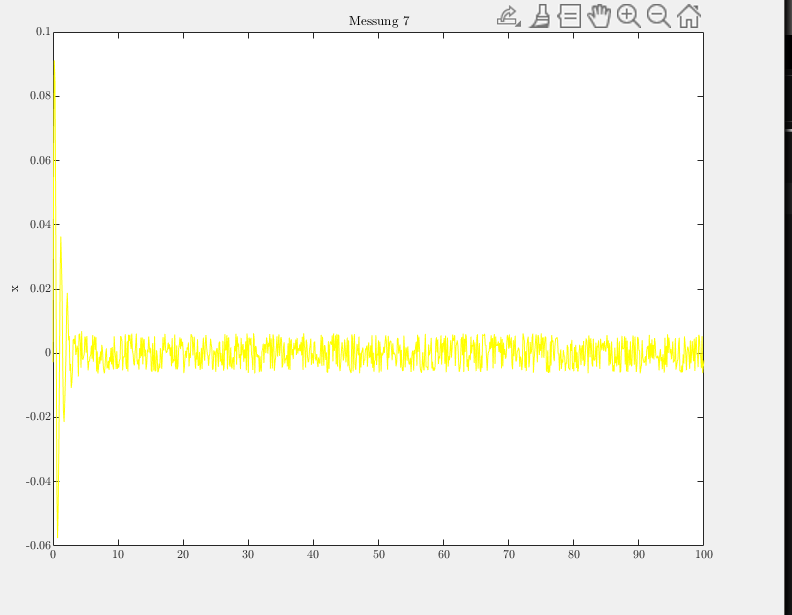
\includegraphics[width=0.5\linewidth]{images/Negativbesipiel_sehr_schlecht}
	\caption{Messung 7}	   	
	\label{fig:negativbeispiel_sehr_schlecht}
\end{figure}

Vergleich mit Simulation aus Vorbereitung zeigt, dass das Ergebnis nicht gleich ist. In der Simulation wurde der Luftwiderstand nicht berücksichtigt, was zur Abweichung führt.

\noindent(Dies dient zur Verdeutlichung, wie es nicht umgesetzt werden soll.)



\section{Bezug zur Laborangabe}\label{sec:bezug_zur_Angabe}
Folgend befindet sich ein besseres Beispiel der selben Aufgabenstellung. Beachten Sie hier, dass der Unterschied erklärt und sogar durch eine angepasste Simulation bestätigt wurde. Das Bild wurde im Text referenziert, die Schriftgröße des Bildes ist ausreichend groß und die Achsen sind beschriftet. Das Bild ist vom Format her so, dass die gesamte Seitenbreite bei geringem vertikalen Platzverbrauch ausgenützt wird. Allgemein soll bei einem Vergleich von Simulation und Messung darauf geachtet werden, dass es wirklich vergleichbar ist. Wenn die Messung mit \SI{100}{\milli\meter} Anfangsauslenkung durchgeführt wird macht es keinen Sinn das mit einer Simulation mit \SI{600}{\milli\meter} Anfangsauslenkung in einer anderen Richtung zu vergleichen. Außerdem soll darauf geachtet werden, dass nur relevante Bereiche im Plot gezeigt werden. Es ist häufig besser, die Zeitachse der Messergebnisse so anzupassen, dass Messungen in den Plots bei $t=0$ beginnen.

\subsection{So schon:}
Um das Modell aus \eqref{eq:bsp_modellgleichung} zu überprüfen wurde ein Ausschwingversuch des Systems durchgeführt. Der Prüfstand wurde dazu um ca. \SI{100}{\milli\meter} ausgelenkt und das Ausschwingen wurde aufgezeichnet. Ein Vergleich mit der Simulation kann aus Abbildung~\ref{fig:simulation_und_messung} entnommen werden.
\begin{figure}[!ht]
	\centering
	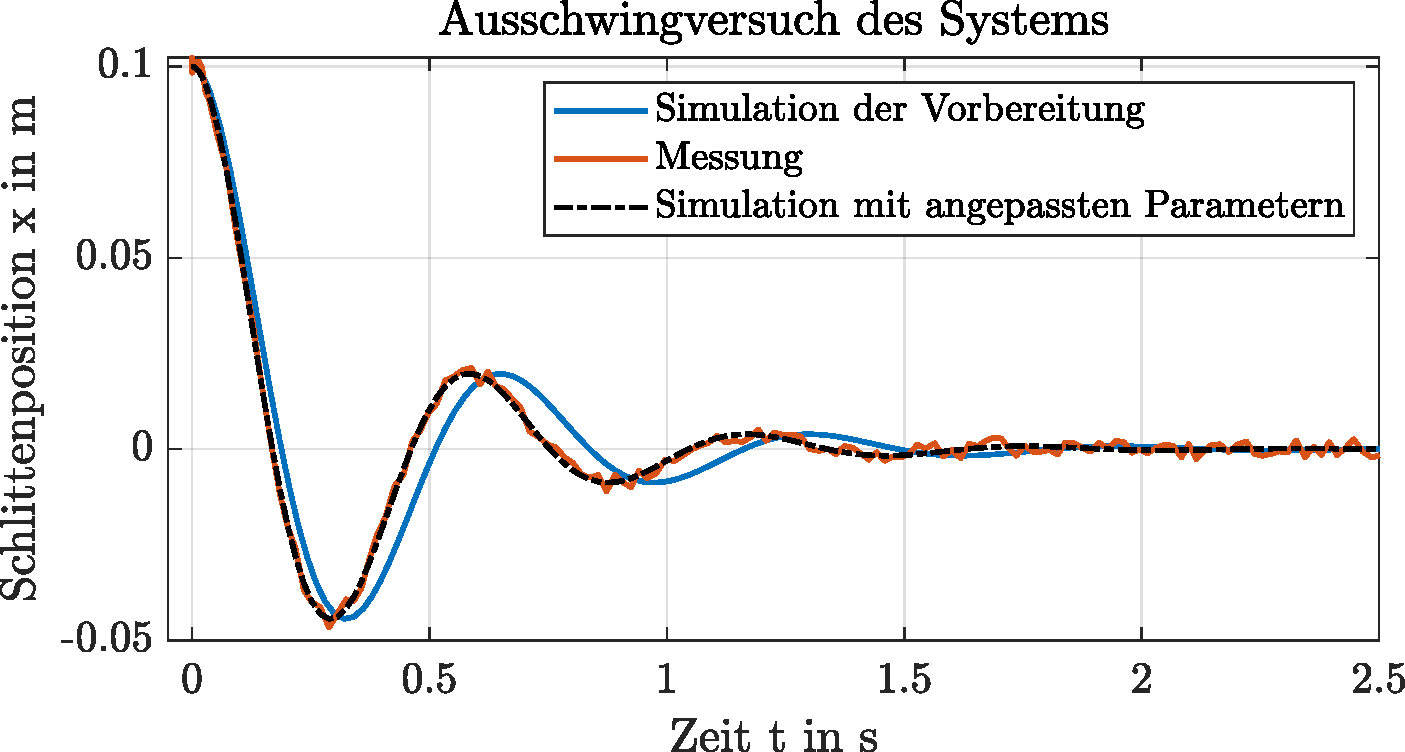
\includegraphics[width=0.95\linewidth]{images/Vergleich_Sim_und_Messung}
	\caption{Vergleich von Messung und Simulation bei einem Ausschwingversuch mit einer Anfangsauslenkung von \SI{100}{\milli\meter}. Die zweite Simulation zeigt, dass eine Abweichung der Parametern zu den Unterschieden zwischen Messung und Simulation führten.}	   	
	\label{fig:simulation_und_messung}
\end{figure}
Ein Vergleich der ursprünglichen Simulation deutet auf Abweichungen der Parameter hin. Um dies zu überprüfen wurde die Federkonstante in der Simulation auf $k=\SI{234}{\newton\per\meter}$ angepasst und die Simulation wurde erneut durchgeführt. Dieser Parameter wurde über mehrere Iterationen der Simulation und durch händisches anpassen ermittelt.



\section{Zusammenfassung/ Diskussion}
Dieses Dokument liefert einen kurzen Überblick und liefert ein Beispiel, wie der Bericht aufgebaut werden soll. Vergleiche mit Berichten von vergangenen Semestern werden zeigen, ob die Punkte beachtet werden. In der Zusammenfassung befindet sich eine Interpretation der Ergebnisse der Laborübung und es ist \underline{keine Erlebniserzählung}. Fassen sie kurz zusammen, was durchgeführt wurde, was die Erkenntnisse daraus waren und was Anknüpfungspunkte für weitere Experimente und Verbesserungen sind. 



%-------------------------------------------------------


% Hier beginnt Ihr Laborbericht 





\bibliography{sources}{}

\end{document}
